% Tento soubor nahraďte vlastním souborem s obsahem práce.
%=========================================================================
% Autoři: Michal Bidlo, Bohuslav Křena, Jaroslav Dytrych, Petr Veigend a Adam Herout 2019
\chapter{Úvod}
TODO

\chapter{Blockchain}\label{chap:blockchain}

Táto kapitola vysvetľuje základné koncepty a pojmy spojené z technológiou blockchain, ako aj samotnú dátovú štruktúru blockchain. Sekcia~\ref{sec:ladger} vysvetľuje pojmi distribuovaná účtovná kniha a blockchain. Ďalej rozoberá vlastnosti a využitie blockchainu. Sekcia~\ref{sec:crypto} vysvetľuje kryptografiu používanú v blockchaine (hashovanie, a asymetrická kryptografia).  Sekcia~\ref{sec:p2p} popisuje peer-to-peer siete a ich využitie v blockchaine. Nazáver sú v sekcii~\ref{sec:data-struct-blockchain} spojené všetky vysvetlené koncepty dokopy a je popísaná samotná dátová štruktúra blockchain.

\section{Distribuovaná účtovná kniha}\label{sec:ladger}
\textit{Účtovná kniha} (anglicky \textit{ledger}) sa v histórii ľudstva dlhodobo používa na záznam rôznych položiek, najčastejšie peňazí a majetku. Príchod digitalizácie a globalizácie presunul tento známy koncept z papierovej podoby do elektronickej. Toto prináša nové výzvy z hľadiska bezpečnosti.
\textit{Distribuovaná účtovná kniha} (anglicky \textit{distributed ledger}) je všeobecne technológia, ktorá poskytuje dôveryhodnú a bezpečnú databázu zdieľanú naprieč viacerými inštitúciami, krajinami a to typicky verejne. Najtypickejším odvetvím využitia distribuovanej účtovnej knihy je bankovníctvo. Banka poskytuje centralizovanú autoritu, ktorá zabezpečuje bezpečnú manipuláciu s peniazmi klientov. Tento koncept označujeme ako centralizovaná účtovná kniha.~\cite{dltUkReport}

V roku 2008 bola publikovaná práca~\cite{satoshiBitcoin}, ktorá navrhla \textit{decentralizovanú} distribuovanú účtovnú knihu. Práca navrhla koncept elektronického platobného systému, ktorého bezpečnosť je založená na kryptografickom dôkaze namiesto dôvere v centralizovanú autoritu. Takáto distribuovaná účtovná kniha sa nazýva \textbf{blockchain}.
\subsection{Vlastnosti blockchainu}
Blockchain je dátová štruktúra, ktorá má nasledujúce vlastnosti:
\begin{itemize}
	\item \textbf{Decentralizácia}: Blockchain funguje nad peer-to-peer sieťou, ktorá nepotrebuje centralizovanú dôveryhodnú autoritu.
	\item \textbf{Auditovateľnosť}: Blockchain v sebe nesie celú histórie zmien jeho obsahu a teda každú zmena stavu dát uložených v blockchaine je možné sledovať.
	\item \textbf{Nemennosť}: Pri správnom použití a dostatočne veľkej sieti nie je možné zmeniť histórie alebo dátový obsah blockchainu.
	\item \textbf{Anonymita}: Užívatelia pracujúci s blockchainom používajú na identifikáciu asymetrickú kryptografiu s digitálnym podpisom. Takýto kryptografický identifikátor neodhaľuje skutočnú identitu užívateľa a pritom umožňuje nepopierateľne určiť vlastníka elektronického zdroja.
\end{itemize}

Tieto vlastnosti blockchainu sú zabezpečené pomocou peer-to-peer siete na ktorej je blockchain postavený (viď sekcia~\ref{sec:p2p}) a taktiež pomocou samotnej dátovej štruktúry, ktorá využíva modernú kryptografiu (viď sekcia~\ref{sec:data-struct-blockchain}).~\cite{horizenAcademy}

\subsection{Aplikačné využitie}

Blockchain bol navrhnutý a po prvýkrát implementovaný za účelom poskytnúť elektronickú peňažnú menu nezávislú od centralizovaného bankovníctva. Tento prvý, a najznámejší, blockchain je Bitcoin~\cite{satoshiBitcoin}. Avšak vlastnosti blockchainovej technológie nachádzajú uplatnenie vo veľkom množstve odvetví. Nasledujúci zoznam vymenúva niekoľko aplikácií, ktoré blockchain môže riešiť~\cite{homoliakBlockchain}:

\begin{itemize}
	\item \textbf{Elektronická peňaženka}: Elektronické peňaženky pre obchod s nejakou formou peňazí (typicky v podobe tokenov). Takéto tokeny sú typicky vlastnené pomocou privátneho kľúča, ktorý má uschovaný majiteľ. Majiteľ môže vlastníctvo tokenov presúvať na iné subjekty v danej sieti.
	\item \textbf{Zmenárne}: V dnešnej dobe existuje veľké množstvo elektoronických peňažných mien postavených nad blockchainom. Takéto meny všeobecne označujeme ako kryptomeny. Z dôvodu veľkého množstva kryptomien sa prirodzene zvyšuje dopyt po zmenárni medzi jednotlivými kryptomenami. Klasická zmenáreň je riešená tradične centralizovanou autoritou. Avšak blockchain je vhodnou technológie aj pre decentralizovanú zmenáreň.
	\item \textbf{Súborové systémy}: V dnešnej dobe už existujú decentralizované súborové systémy založené na peer-to-peer sieťach. Implementácia takéhoto decentralizovaného súborového systému ako blockchain by nám umožnila nepopierateľne a trasovateľne verzovať zmeny v obsahu.
	\item \textbf{Správa identít}: Správa identít je typicky centrálna autorita, ktorá prideľuje pre konkrétne entity určité zdroje na ktoré majú právo. Ide o schému podobnú banke. Blockchain by v tomto prípade opäť umožnil náhradu tejto centralizovanej autority za decentralizovanú sieť.
	\item \textbf{Voľby}: Elektronické voľby sú ďalším vhodným príkladom, kde sa dá efektívne využiť blockchain. Voliace entity predstavujú decentralizovanú sieť a vlastnosti blockchainu zase poskytujú transparentnosť a verejnú overiteľnosť.
	\item \textbf{Reputačné systémy}: Reputačné systémy slúžia na meranie úrovne dôvery v určité entity. Typickým príkladom je reputácia rôznych predajcov na základe hlasovania zákazníkov. Transparentnosť a nemennosť blockchainovej histórie by znížila možnosť manipulácie s reputáciu v prospech nejakej entity.
	\item \textbf{Aukcie}: Elektronická aukcia je služba veľmi podobná elektronickej peňaženke alebo zmenárni s podobnými bezpečnostnými požiadavkami. Tieto vlastnosti by opäť dokázala pokryť technológia blockchain.
\end{itemize}

\section{Kryptografia v blockchaine}\label{sec:crypto}
Pre pochopenie technológie blockchain je potrebná základná znalosť modernej kryptografie. V tejto sekcii je popísaný kryptografická hashovacia funkcia (pozri~\ref{subsec:hash}) a jej využitie na tvorbu dátových štruktúr zabezpečených proti modifikácii obsahu (viď sekcia~\ref{subsec:hash-pointer}). Ďalej je vysvetlený koncept asymetrickej kryptografie a digitálneho podpisu (viď sekcia~\ref{subsec:sign}). Tieto kryptografické primitíva sú základom na ktorom stojí nemennosť, auditovateľnosť a anonymita blockchainu.

\subsection{Hashovacia funkcia}\label{subsec:hash}
Hashovacia funkcia je taká funkcia $h$, ktorá má ako parameter $x$ reťazec bitov ľubovolnej dĺžky a vracia reťazec $y$ s konštantnou dĺžkou(viď rovnica~\ref{eq:hash}). Reťazec $y$ voláme hash. Hashovacia funkcia vracia pre konkrétny vstup vždy rovnaký hash.

\begin{equation} \label{eq:hash}
	h(x) = y
\end{equation}
Kryptografická hashovacia funkcia, alebo tiež jednocestná funkcia (anglicky \textit{one way function}), je taká hashovacia funkcia pre ktorú platia nasledujíce tri vlastnosti:
\begin{enumerate}
	\item Pre daný hash $x$ je výpočetne nezvládnuteľné nájsť správu takú, že $ h(x) = y $. Anglicky voláme túto vlastnosť \textit{first preimage resistant}.
	\item Pre danú správu je výpočetne nezvládnuteľné nájsť inú správu s rovnakým hashom. Anglicky voláme túto vlastnosť \textit{second preimage resistant}.
	\item Pre ľubovoľnú správu je výpočetne nezvládnuteľné nájsť inú správu s rovnakým hashom. Anglicky voláme túto vlastnosť \textit{collision resistant}.
\end{enumerate}

Hashovacie funkcie majú v oblasti počítačovej bezpečnosti dôležité využitie:
\begin{itemize}
	\item Bezpečné ukladanie hesiel: Digitálna služba neukladá v databáze heslo, ale len jeho hash. Pri ukradnutí databázy nedochádza k odhalenie hesiel užívateľov.
	\item Integrita dát: Hashovacia funkcia môže byť použitá na ochranu integrity ľubovoľných dát. Ak spočítate hash veľkého súboru a bezpečne ho uložíte tak ste schopný detekovať, že niekto tento súbor zmenil.
	\item Digitálny podpis: Hashovacia funkcia je kryptografické primitívum potrebné pre vytvorenie digitálneho podpisu.
\end{itemize}
Existuje množstvo hashovacích funkcií. Medzi veľmi známe a používané patrí napríklad MD5 (128 bitový výstup), SHA256 (256 bitový výstup), SHA512 (512 bitový výstup).~\cite{cryptoHandbook, nigelSmartCrypto}

\subsection{Hash ukazovateľ}\label{subsec:hash-pointer}
Hash ukazovateľ (anglicky \textit{hash pointer}) je primitívom pre tvorbu dátových štruktúr s kryptografickým zabezpečením proti manipulácia s obsahom (anglicky \textit{tamper-evident}). Hash ukazovateľ funguje ako klasický ukazovateľ v zozname či strome. Navyše však neumožňuje meniť už pridané prvky. Jediná povolená operácia je pridanie ďalšieho prvku do dátovej štruktúry. 

Obrázok~\ref{img:hash-pointer} demonštruje rozdiel medzi zoznamom vytvoreným pomocou klasických ukazovateľov a pomocou hash ukazovateľov. Bežný zoznam umožňuje pozmeniť ľubovoľný už existujúci prvok nezávisle na zvyšku zoznamu. Naopak, hash pointer referencuje pomocou samotného dátového obsahu. Ak by sme zmenili dátový obsah prvku B, tak by sa narušila referencia v predchádzajúcom prvku.
~\cite{horizenAcademy, narayanan2016bitcoin}


\begin{figure}[bt]
	\centering
	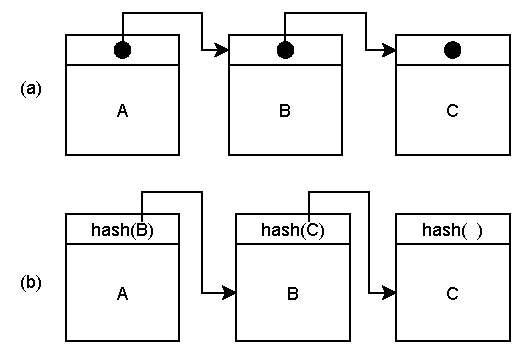
\includegraphics[width=.6\textwidth]{obrazky-figures/hash-pointer}
	\caption{(a) Zoznam pomocou ukazovateľov \medspace (b) Zoznam pomocou hash ukazovateľov}
	\label{img:hash-pointer}
\end{figure}

\subsection{Digitálny podpis}\label{subsec:sign}
Digitálny podpis (anglicky \textit{digital signature}) je kryptografický koncept používaný na autentifikáciu, autorizáciu a nepopierateľnosť. Digitálny podpis jednoznačne prepojí určitú entitu s informáciu. V technológii blockchain slúži digitálny podpis na určenie vlastníctva zdrojov, ktoré blockchain uchováva.~\cite{cryptoHandbook, satoshiBitcoin}

Moderná kryptografia používa pre zaistenie dôvernosti šifrovanie pomocou tajného kľúča. Pre zašifrovanie a dešifrovanie tajnej správy je potrebná znalosť tajného kľúča. Tento mechanizmus  zaisťuje dôvernosť avšak nezaisťuje nepopierateľnosť pretože obe komunikujúce strany poznajú tajný kľúč a teda nie je možné právne dokázať kto správu napísal. Na zaistenie nepopierateľnosti sa používa asymetrické šifrovanie, ktoré používa dvojicu kľúčov:
\begin{itemize}
	\item \textbf{Privátny kľúč} je tajný a pozná ho len odosielateľ správy. Odosielateľ používa tento kľúč na zašifrovanie správy.
	\item \textbf{Verejný kľúč} je dostupný komukoľvek. Ktokoľvek s týmto kľúčom dokáže dešifrovať správu.
\end{itemize}
Tieto dva kľúče tvoria dvojicu prepojenú matematickým spôsobom. Zo znalosti verejného kľúča je výpočetne nezvládnuteľné zistiť privátny kľúč. Zašifrovaná správa nie je dôverná pretože ktokoľvek môže použiť verejný kľúč na jej dešifrovanie. Avšak zašifrovaná správa je nepopierateľne napísaná vlastníkom privátneho kľúča. 

Tento koncept je základom digitálneho podpisu. Ak chceme nepopierateľne dokázať, že nejaký dátový obsah (napríklad pdf dokument) sme vytvorili mi, tak vypočítame jeho hash (viď sekcia~\ref{subsec:hash}) a zašifrujeme ho naším privátnym kľúčom. Zašifrovaný hash priložíme k dokumentu. Príjemca dokumentu si následne pomocou verejného kľúča dešifruje hash priložený k správe a porovná si ho s tým ktorý vypočítal sám z danej správy. Ak sú hashe rovnaké tak nikto správu nezmenil a dokument je jednoznačne vytvorený vlastníkom tajného kľúča. Najznámejšie algoritmy na digitálny podpis sú RSA, DSA, ECDSA.~\cite{cryptoHandbook}

\subsection{Prahový digitálny podpis}\label{subsec:threshold-sig}
Prahový digitálny podpis (anglicky \textit{threshold signatures}) je špeciálna schéma digitálneho podpisu. V tejto schéme je $n$ účastníkov a každý vlastní časť privátneho kľúča. Každý účastník môže použiť svoju časť tajného kľúča na čiastočné podpísanie správy $M$. Kompletný podpis môže byť zostrojený ak aspoň $t$ účastníkov poskytlo svoju časť podpisu. Potom hovoríme o  $t$-z-$n$ prahovom podpise. Takýto koncept sa dá využiť pri kryptografickom hlasovaní.~\cite{blsSignature}


\section{Peer-to-peer sieť}\label{sec:p2p}

Technológia blockchain je postavená na peer-to-peer sieťach. Peer-to-peer sieť sa podieľa na decentralizovanosti, nemennosti a auditovateľnosti blockchainu. 

Peer-to-peer sieť je dynamický súbor nezávislých uzlov (anglicky \textit{peers}), ktoré sú prepojené do grafu. Každý uzol obsahuje zdroje, ktoré zdieľa všetkým ostatným uzlom v sieti.~\cite{p2pBuford, p2pSchollmeier} Dôvod existencie peer-to-peer sietí je teda decentralizovaný spôsob zdieľania zdrojov ako sú súbory, fyzické zariadenia, výpočetný výkon alebo aj elektronické finančné zdroje. Dnes existuje množstvo peer-to-peer sietí. Veľmi známe sú napríklad Gnutella, Kazaa alebo BitTorrent.~\cite{p2pEssence}

\subsection{Referenčný model}
Najbežnejšie technické riešenie peer-to-peer siete je navrstvenie siete (anglicky \textit{overlay network}) na už existujúcu sieť, ktorou je typicky Internet. Takúto sieť potom môžeme definovať ako päticu $(P,R,I,F_P,F_R)$, kde:
\begin{itemize}
	\item $P$ je množina uzlov
	\item $R$ je množinu zdrojov
	\item $I$ je priestor identifikátorov
	\item $F_P: P \rightarrow I$ je funkcia, ktorá mapuje uzoly na identifikátory
	\item $F_R: R \rightarrow I$ je funkcia, ktorá mapuje zdroje na identifikátory
\end{itemize}

Obrázok~\ref{img:p2p-ref-model} ukazuje princíp fungovania takto definovanej siete. Tvorba siete s týmto modelom je potom závislá od šiestich návrhových aspektov:
\begin{enumerate}
	\item Voľba priestoru identifikátorov.
	\item Mapovanie zdrojov a uzlov na identifikátory.
	\item Správa priestoru identifikátorov v réžii uzlov siete.
	\item Tvorba grafu (štruktúra siete).
	\item Stratégia smerovania (anglicky \textit{routing}).
	\item Stratégia údržby.
\end{enumerate}
Konkrétne riešenie pre popisovaných šesť aspektov je zavislé od požiadaviek na efektivitu, škálovateľnosť, samoorganizovateľnosť, odolnosť voči chybám a kooperáciu.~\cite{p2pEssence}

\subsection{Využitie v blockchaine}

Peer-to-peer sieť umožňuje blockchainu uchovávať jeho obsah decentralizovane a pritom bezpečne. Tento koncept si vysvetlíme na prípade blockchainu, ktorý sa využíva ako kryptomena.

Elektronické financie sú typicky reprezentované pomocou elektronických mincí. Takáto minca je reprezentovaná pomocou nejakej sekvencie bitov. Avšak narozdiel od fyzických mincí, elektronické mince umožňujú jednoduchú falzifikáciu. Útočník skopíruje bitový reťazec danej mince a zaplatí ním viacnásobne rôzne produkty. Tento útok sa volá zdvojnásobenia výdavkov (anglicky \textit{double-spending attack}). Proti tomuto útoku existuje tradičné zabezpečenie pomocou centrálnej autority. Banka je centrálna autorita, ktorá schvaľuje všetky manipulácie s elektronickými mincami a teda neumožní použiť mincu takýmto podvodným spôsobom. Avšak toto riešenie nie je možné použiť v decentralizovanej sieti, kde centrálna autorita neexistuje. V prípade decentralizovanej siete je možné zabrániť tomuto útoku pomocou použitia dátovej štruktúry blockchain.~\cite{doubleSpending}

Kryptomena Bitcoin ako prvá navrhla použitie peer-to-peer siete v spojení s blockchain technológiou pre zabránenie double-spending útoku. V takejto sietu je jediný zdroj na zdieľanie a to je dátová štruktúra blockchain v ktorej sú uložené všetky informácie o elektronických financiách. Zjednodušene môžeme povedať, že majorita uzlov siete zdieľa rovnaký zdroj (rovnakú kópiu blockchainu). Ak chce niektorý uzol vykonať finančnú transakciu tak zašle správu s navrhovanou zmenou blockchainu do siete. Uzly v tejto sieti nie je potrebné identifikovať pretože správy posielané v tejto sieti nie sú smerované na žiadne konkrétne miesto. Keď uzol prijme správu s nejakou modifikáciu tak si overí či ide o validnú požiadavku na finančnú transakciu. Štruktúra blockchainu používa modernú kryptografiu na overenie validnosti transakcie (pozri sekciu~\ref{sec:crypto}). Blockchain, ktorý vlastní väčšina siete je ten, ktorý sa považuje za pravdu. Útočník by musel teda vlastniť aspoň 51\,\% uzolov v sieti aby mohol vykonať double-spending útok. Ak je daná sieť dostatočne veľká tak by toho útočník nemal byť schopný dosiahnuť.~\cite{satoshiBitcoin}

\begin{figure}[bt]
	\centering
	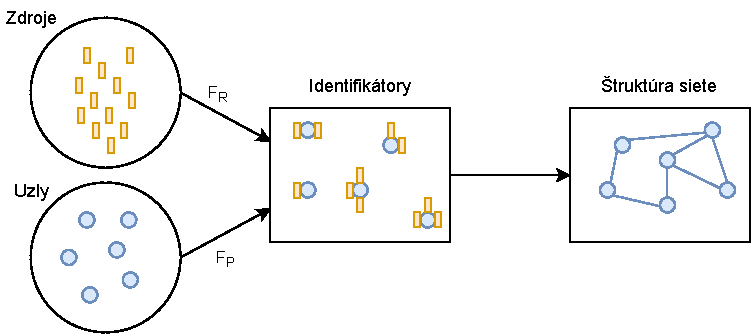
\includegraphics[width=\textwidth]{obrazky-figures/p2p-ref-model.pdf}
	\caption{Referenčný model peer-to-peer siete.~\cite{p2pEssence}}
	\label{img:p2p-ref-model}
\end{figure}

\section{Datová štruktúra blockchain}\label{sec:data-struct-blockchain}
Blockchain je dátová štruktúra podobná zoznamu (anglicky \textit{linked list}). Blockchain organizuje dáta do podmnožín, ktoré sa volajú bloky. Blok je podobný uzlu v zozname. Každý blok obsahuje referenciu na ďalší blok. Rozdiel medzi zoznamom a blockchainom je v tom, že referencia blockchainu je zabezpečená proti manipulácia (anglicky \textit{tamper-evident}) pomocou modernej kryptografie. Bežný zoznam používa referenciu pomocou ukazovateľov (anglicky \textit{pointers}), ktoré môže ktokoľvek a kedykoľvek pozmeniť bez toho aby pozmenil dátový obsah. Naopak, blockchain vôbec neumožňuje meniť už pridané bloky. Jediná povolená operácia je pridanie ďalšieho bloku na koniec blockchainu.~\cite{horizenAcademy}

Každý blok obsahuje dáta, ktoré sú typicky vo forme transakcií. Kryptograficky bezpečný blockchain by mohol fungovať aj tak, že v každom bloku bude uložená práve jedna transakcia. Z dôvodu optimalizácie je ale v jednom bloku uložené množstvo transakcií. Vďaka tejto optimalizácii nemusí celá sieť vytvárať konsenzus po každej transakcii. Samotné transakcie v rámci jedného bloku sú ukladané v ďalšej dátovej štruktúre, ktorá taktiež používa kryptografické hashovanie (viď sekcia~\ref{subsec:merkle-tree}).~\cite{narayanan2016bitcoin}

\subsection{Blok}\label{subsec:block}

Blok sa skladá z hlavičky a tela. Telo bloku obsahuje dáta a hlavička obsahuje metadáta. Dáta v tele bloku sú uložené vo forme transakcií. Transakcie sú popísané v sekcii~\ref{subsec:transaction}. Počet transakcií v bloku je typicky obmedzený maximálnou veľkosťou bloku.
Hlavička bloku obsahuje metadáta o bloku, kde najdôležitejšie a najbežnejšie sú nasledujúce:
\begin{itemize}
	\item Hash všetkých transakcií.
	\item Časové razítko vytvorenia bloku.
	\item Hash ukazovateľ na predošlý blok v blockchaine.
	\item Náhodná výzva (anglicky \textit{nonce}), ktorej využitie vysvetľuje sekcia~\ref{subsec:pow}
\end{itemize} 

~\cite{zhengBlockchainOverview}


\subsection{Transakcia}\label{subsec:transaction}
Transakcia je elementárna dátová jednotka na ukladanie dáta v blockchaine. Bitcoin, prvý blockchain, použil transakciu na manipuláciu s elektronickými financiami. Takáto transakcia sa skladá z troch častí:
\begin{itemize}
	\item \textbf{Množina vstupov}: Každý vstup má uložený hash predošlej transakcie s ktorej vychádza. Ďalej definuje, ktoré výstupy s predošlej transakcie si nárokuje. Nakoniec obsahuje digitálny podpis, ktorý autorizuje tvorcu transakcie.
	\item \textbf{Množina výstupov}: Každý výstup má hodnotu, ktorá je uchovávaná v blockchaine (typicky minca nejakej kryptomeny). Suma hodnôt všetkých výstup transakcie musí byť menšia alebo rovná sume všetkých vstupov transakcie. Ak je menšia, tak tento rozdiel je použitý ako odmena pre toho, kto publikoval tento blok blockchainu.
	\item \textbf{Hlavička}: Obsahuje hash transakcie, ktorý je používaný ako unikátny identifikátor pomocou, ktorého sa na transakciu odkazujeme.
\end{itemize}


\subsection{Binárny hashovací strom}~\label{subsec:merkle-tree}
Binárny hashovací strom alebo tiež Merkle strom (anglicky \textit{Merkle tree}) je datová štruktúra podobná binárnemu stromu, ktorá slúži na efektívne a rýchle vypočítanie hashu veľkého množstva dát. Blockchain používa tento strom na časovo efektívny výpočet hashu všetkých transakcií. Takto vypočítaný hash je uložený v hlavičke bloku.

Merkle strom je vyvážený binarny strom, kde listové uzly obsahujú jednotlivé transakcie uložené v danom bloku blockchainu. Každý nelistový uzol stromu obsahuje hash vypočítaný z jeho potomkov. Koreňový uzol teda obsahuje hash celého stromu a teda aj všetkých transakcií. Pridanie, odobranie, zmena obsahu, alebo zmena poradia transakcií bude teda viesť k zmene koreňového hashu. Konštrukcia stromu, inak povedané výpočet hashu všetkých transakcií, prebieha následovne:
\begin{enumerate}
	\item Všetky transakcie sú uložené do listovej úrovne stromu. Ak je počet transakcií nepárny tak, je posledná vložená dvakrát.
	\item Nad každým listovým uzlom je vypočítaný hash.
	\item Každý nelistový uzol skonkatenuje hash ľavého a pravého syna, vypočíta nad nimi hash a uloží si ho. 
\end{enumerate}
Konštrukcia takéhoto stromu pre $n$ transakcií má časovú zložitosť $O(log(n))$. Takýto spôsob výpočtu hashu je teda veľmi efektívny pre veľké množstvo transakcií (blok v blockchaine bežne obsahuje stovky transakcií).~\cite{merkleTreeBosamia}

Merkle strom umožnuje efektívne šetriť pamäťové nároky blockchainu. Do blockchainu sú neustále pridávané nové bloky, ktoré obsahujú aj rovnaké staré transakcie. Ak už sú transakcie zaznamenané v dostatočne veľkom množstve blokov tak sú z hľadiska bezpečnosti nemenné. V nových blokoch ich už preto nie je potrebné ukladať. Nový blok si preto uloží len hashe starých vetiev stromu, ale ich obsah už nepotrebuje. Takto je zachovaná integrita hashu všetkých transakcií.~\cite{satoshiBitcoin}

\section{Ťažba blokov}\label{sec:mining}

Ťažba (anglicky \textit{mining}) bloku je proces pridania nové bloku na koniec blockchainu. Ťažba bloku zahŕňa validáciu transakcií a blokov. Preto je ťažba kritická pre správne a bezpečné fungovanie blockchainu. Každý uzol siete, ktorý ťaží nové bloky sa nazýva anglickým slovom \textit{miner}. Tieto uzly umožňujú rozširovanie blockchainu. Aby takéto uzly existovali, musia byť motivované. Miner dostane za každý vyťažený blok ako odmenu zdroje uložené v blockchaine.

Ťažba všeobecne pozostáva z nasledujúcich krokov:
\begin{enumerate}
	\item Miner prijíma požiadavky na transakcie z peer-to-peer siete. Každú transakciu si validuje pomocou kryptografie popísanej v sekcii~\ref{sec:crypto}.
	\item Miner musí taktiež udržiavať aktuálny stav blockchainu. Je potrebné sledovať či nevznikli nové bloky a udržiavať si validný blockchain.
	\item Ak miner vlastní validnú a aktuálnu kópiu blockchainu, môže začať vytvárať nový blok. Do nového bloku vloží transakcie, ktoré prijal a boli validné.
	\item Novo vytvorený blok je potrebné distribuovať do siete. Ak väčšina siete blok získa a akceptuje, tak bol pridaný do blockchainu. Tento proces zahŕňa problém konsenzu v sieti, ktorý je podrobne vysvetlený v sekcii~\ref{sec:consenzus}.
	\item Ak sa podarilo úspešne blok pridať do blockchainu tak miner získava odmenu. Odmena za vyťažený blok je konštantná čiastka zdrojov poskytovaných daným blockchainom. Napríklad Bitcon poskytuje v roku 2021 ako odmenu 6,25 bitcoinov čo približne 300 dolárov~\footnote{\url{https://www.investopedia.com/tech/how-does-bitcoin-mining-work/}}. Avšak táto odmena môže byť navýšená o poplatky, ktoré sú v transakciách. Ak teda chcete aby sa vaša transakcia dostala do blockchainu čo najrýchlejšie, poskytnete vyššiu odmenu v podobe poplatku za transakciu. Miner bude potom viac motivovaný pridať práve túto transakciu do bloku.
\end{enumerate}

~\cite{narayanan2016bitcoin}

\section{Konsenzus}\label{sec:consenzus}
Konsenzus v blockchaine zabezpečuje, že skupina uzlov (peerov) sa  zhodne na rovnakom stave blockchainu. Tradične je konsenzus zabezpečený centrálnou autoritou s ktorou musia byť všetky uzly spojené. Avšak blockchain je decentralizovaný a teda toto riešenie nie je možné. Konsenzus v decentralizovanej sieti blockchainu je zabezpečený pomocou protokolu, ktorý sa snaží nájsť kompromis medzi nasledujúcimi vlastnosťami~\cite{gilbertCAP, zhangConsensus, leporeConsensus}:
\begin{itemize}
	\item Konzistentnosť: Vždy keď dôjde k potvrdeniu zmeny, celý reťazec sa aktualizuje a všetci čítajú rovnaké hodnoty.
	\item Dostupnosť: Pre každú požiadavku na dáta musí byť poskytnutá odpoveď.
	\item Odolnosť voči prerušeniu (anglicky \textit{partial tolerance}): Sieť funguje aj v prípade, že v nej vznikajú chyby.
\end{itemize}

Existujú tri najbežnejšie techniky, ktoré sa používajú pre ustavenie konsenzu~\cite{homoliakBlockchain}:
\begin{itemize}
	\item \textbf{Lotéria}: Takéto protokoly náhodne zvolia uzol, ktorý vyprodukuje nový blok. Výhodou tohoto prístupu je jeho jednoduchosť keďže takýto proces nevyžaduje žiadnu interaktivitu. Nevýhodou tohoto prístupu je, že pripúšťa možnosť voľby viacerých uzlov súčasne. V takom prípade sa reťazec rozvetví (anglicky \textit{fork}) a je potrebné určiť ktorá vetva je správna. Typicky sa za správnu vetvu volí tá najdlhšia. Avšak takéto správanie oslabuje konzistentnosť blockchainu. Transakcie v posledných blokoch môžu byť potenciálne zahodené pretože nejde o správnu vetvu. Preto sa za konzistentné transakcie považujú až tie ktoré sú prekryté väčším množstvom nových blokov.
	\item \textbf{Hlasovanie}: Protokoly založené na hlasovaní dosahujú dohodu pomocou hlasovania všetkých zapojených uzlov. Môžeme použiť napríklad protokol Byzantskej chyby (anglicky \textit{Byzant fault tolerance}), ktorý vyžaduje majoritu hlasov k uzavretiu konsenzu (typicky $\frac{2}{3}$). Výhodou je veľmi malá pravdepodobnosť vzniku vetiev reťazca. Na druhej strane, takéto protokoly majú nižšiu priepustnosť, ktorá klesá z narastajúcim počtom uzlov.
	\item \textbf{Kombinovaný prístup}: Tieto protokoly sa snažia kombinovať prístup lotérie a hlasovania s cieľom dosiahnuť výhody oboch prístupov. Napríklad je možné rozdeliť počet uzlov podieľajúcich sa na hlasovaní pomocou lotérie, čím sa zvýši priepustnosť.
\end{itemize}
~\cite{zhangConsensus, homoliakBlockchain}

\subsection{Proof-of-Work}\label{subsec:pow}
Dôkaz prácou (anglicky \textit{proof of work}) je najbežnejšia stratégia konsenzus protokolu. Ak chce uzol publikovať nový blok, musí investovať svoj výpočtový výkon do riešenia netriviálneho kryptografického problému. Uzol, ktorý ako prvý vyrieši tento problém má najväčšiu pravdepodobnosť, že bude jeho blok pridaný do reťazca. Samozrejme, je tu možnosť, že problém vyrieši súčasne viacero uzlov. Konečná voľba je teda náhodná. Proof-of-work teda umožňuje, aj keď s oveľa menšou pravdepodobnosťou, že sa reťazec rozvetví. Bezpečnosť takéhoto konsenzu spočíva v tom, že majorita výpočtového výkonu siete (51\,\%) je vlastnená poctivými uzlami.~\cite{leporeConsensus}

Samotný kryptografický problém, ktorý sa rieši spočíva v počítaní hashu (viď~\ref{subsec:hash}) z hlavičky nového bloku (viď~\ref{subsec:block}). Hlavička obsahuje atribút nonce, ktorý môže miner ľubovolne nastaviť. Zmenou tohoto atribútu môže miner získať iný hash hlavičky bloku. Konsenzus vyžaduje aby výsledná hash hodnota bola menšia rovná určitej zvolenej hodnote. Miner môže túto podmienku dosiahnuť len tak, že bude inkrementovať hodnotu atribútu nonce až dokedy túto podmienku nesplní. Táto úloha sa teda dá riešiť len pomocou metódy útok hrubou silou (anglicky \textit{brute force}). Miner môže svoju šancu na úspech zvýšiť len tým, že poskytne väčší výpočtový výkon do jej riešenia. Na druhej strane, ostatné uzly môžu overiť, že jeho riešenia je správne veľmi rýchlo a efektívne.~\cite{zhengBlockchainOverview}

Proof-of-work konsenzus využíva dva typy uzlov. Prvý typ uzla je miner, ktorý vytvára nové bloky tak ako je popísané v sekcii~\ref{sec:mining}. Druhý typ uzla je bežný vlastník zdrojov v danom blockchaine, ktorý môže vytvárať transakcie a distribuovať ich do siete. Druhý typ uzla teda nehrá žiadnu rolu v ustanovovaní konsenzu.~\cite{leporeConsensus}

Proof-of-work je overený konsenzus protokol, ktorý funguje a používa sa v blockchainoch ako je Bitcoin~\cite{satoshiBitcoin} alebo Ethereum~\footnote{\url{https://ethereum.org/en/whitepaper/}}. Tento protokol má však jeden dlhodobý problém a to je spotreba energie. Uzly ktoré riešia kryptografický problém pre nové bloky spotrebujú veľké množstvo energie čo má nepriaznivý dopad na životné prostredie. Niektoré zdroje~\footnote{\url{https://www.businessinsider.com/bitcoin-mining-electricity-usage-more-than-google-2021-9}} napríklad hovoria, že v roku 2021 pokrýva ťažba Bitcoinu 0,5\,\% celkovej spotreby elektrickej energie na svete. Pre porovnanie, ide o sedemkrát väčšiu spotrebu energie ako má celá spoločnosť Google.~\cite{leporeConsensus}

\subsection{Proof-of-Stake}\label{subsec:pos}

Dôkaz podielom na vlastníctve (anglicky \textit{proof of stake}) je založený na technike lotérie, kde pravdepodobnosť výhry rastie s množstvom už vlastnených zdrojov. Základnou myšlienkou, je že vlastník veľkého množstva zdrojov v danom blockchaine je veľmi nepravdepodobným útočníkom pretože svoje zdroje nechce ohroziť. Uzly sa teda musia preukázať vlastníctvom zdrojov v danom blockchaine ak chcú publikovať nový blok. Pravdepodobnosť výberu uzlu rastie s množstvom zdrojov, ktoré v sieti vlastní.~\cite{homoliakBlockchain, nguyenPos}

Veľkou výhodou proof-of-stake oproti proof-of-work je, že nevyždauje také veľké množstvo energie. Uzly už nemusia súťažiť v riešení výpočtovo náročných úloh. ~\cite{leporeConsensus}

\chapter{Viacvrstvová abstrakcia}

Existuje veľké množstvo blockchain protokolov, ktoré majú rôzne využitie a implementáciu. Avšak všetky tieto implementácie sú založene na spoločnom koncepte distribuovanej účtovnej knihy. Pre ich jednotnú klasifikáciu použijeme nasledujúci model abstrakcie so štyrmi vrstvami:~\cite{homoliakBlockchain}

\begin{enumerate}
	\item \textbf{Sieťová vrstva} predstavuje najnižšiu vrstvu abstrakcie a zaoberá sa peer-to-peer sieťou. Sieť rieši pripájanie nových peerov a komunikácia medzi uzlami v sieti (šírenie transakcií a blokov). Táto vrstva má kritický dosah na výkonnosť blockchainu. Napríklad, verejný blockchain ako je Bitcoin tvorí veľmi rozsiahlu sieť s tisíckami aktívnych uzlov. V takejto sieti sa už vlastnosti ako stratovosť paketov alebo priepustnosť nezanedbateľne prejaví na rýchlosti a stabilite celého blockchainu.~\cite{fanPerfEval}
	\item \textbf{Konsenzus vrstva} definuje protokol pomocou, ktorého sa ustavuje dohoda na stave blockchainu. Táto vrstva kľúčovo ovplyvňuje priepustnosť transakcií (\textit{TPS - transaction per second}). Táto metrika je kľúčová napríklad v oblasti kryptomien. Pre porovnanie, centralizovaný platobný systém VISA~\footnote{\url{https://towardsdatascience.com/the-blockchain-scalability-problem-the-race-for-visa-like-transaction-speed-5cce48f9d44}} má TPS približne 1\,500 zatiaľ čo Bitcoin približne 5.
	\item \textbf{Dátová vrstva} (alebo tiež úložisko) definuje model transakcií (binárny hashovací strom, hashovacie a kryptografické algoritmy).
	\item \textbf{Aplikačná vrstva} definuje využitie v konkrétnej službe (napríklad kryptomena).
\end{enumerate}

\chapter{Útoky na konsenzus}

\section{Všeobecné utoky}

\subsection{Ovládnutie konsenzu útočníkmi}
Tieto útoky narušia decentralizované siete tým, že útočníci dokážu utvoriť konsenzus. V takom prípade sa stáva sieť centralizovaná, kde centrálnou autoritou sú práve útočníci. Príkladom takéhoto útoku pre proof-of-work a proof-of-stake konsenzus je ovládnutie 51\,\% siete. V prípade protokolov Byzantskej chyby dokáže $\frac{1}{3}$ uzlov spôsobiť, že bude protokol narušený alebo dokonca zastavený.~\cite{homoliakBlockchain}

\subsection{Porušenie synchronného doručovania}

Ak útočník dokáže narušiť synchrónne doručovanie správ v protokole, ktorý synchronizáciu predpokladá tak takýto protokol prestane fungovať. Tento útok už nie je možné urobiť na protokole, ktorý umožňuje asynchronnú komunikáciu. Tento útok je možné vykonať napríklad pre protokoly Byzantskej chyby.~\cite{homoliakBlockchain}

\subsection{Útok na časovú synchronizáciu}
Okrem času celého systému majú jednotlivé uzly v sieti vlastný čas. Uzly ho vypočítavajú ako medián všetkých časov získaných od ostatných. Ak je uzol miner tak typicky vloží práve tento čas do hlavičky bloku, ktorý vytvoril. Ostatné uzly v sieti budú pri distribúcii bloku overovať, že čas je dostatočne čerstvý aby bol akceptovaný. Ak útočník disponuje veľkým množstvom uzlov v sieti, tak môže narušiť synchronizáciu času, ktorý bloky získavajú mediánom. Tento útok následne spomaľuje sieť pretože bloky distribuujú bloky s časovou značkou, ktorá už nebude akceptovaná.

\subsection{Zdvojnásobenie výdavkov}

Zdvojnásobenie výdavkov (anglicky \textit{double spending}) je útok, ktorý vzniká vytvorením dvoch alebo viac konfliktných blokov. Tieto bloky vytvárajú tzv. vetvy (anglicky \textit{forks}). S tohoto dôvodu môžu byť niektoré krypto mince dočasne minuté v oboch konfliktných blokoch. Neskôr je síce len jeden z nich validný pretože druhá vetva bude zahodená. Avšak tento útok spomaľuje konzistentnosť blockchainu.

\subsection{Útok na podskupiny uzlov}

Niektoré konsenzus protokoly rozdeľujú celú sieť na podskupiny uzlov (anglicky \textit{shards}). Sharding zvyšuje škálovateľnosť a priepustnosť siete pretože uzly validujú transakcie len v rámci svojej podskupiny. Na druhej strane, tento prístup môže viesť k zníženie bezpečnosti. Množstvo spolupracujúcich uzlov v jednej takejto podskupine je oveľa menší než v celej sieti. Pre útočníka môže byť preto jednoduchšie ovládnuť takúto podskupinu ako celú sieť.

\section{Útoky na proof-of-stake}

\subsection{Vetvenie bez rizika straty zdrojov}
Generovanie blokov v proof-of-stake nestojí žiadnu energiu v podobe výpočtového výkonu. Uzly preto môžu generovať viacero konfliktných uzlov súčasne a tým zvyšovať pravdepodobnosť, že bude práve ich uzol pridaný do reťazca. Takéto správanie nepredstavuje pre daný uzol žiaden risk v podobe straty zdrojov. Problémom tohoto správania je, že vzniká väčšie množstvo vetiev reťazca. Ako dôsledok sa potom zvyšuje čas do konzistentnosti blockchainu.

\subsection{Ovplyvnenie volieb}
Útočník ovplyvňuje voľby v jeho prospech. Takto zvyšuje pravdepodobnosť, že bude zvolený práve jeho blok. 

\subsection{Odmietnutie služby lídrovi/výboru}

Tomuto vobec nerozumiem TODO - najst vhodno literaturu kde sa to vysvetluje

\subsection{Neskoršia korupcia}
Útočník sa snaží získať privátne kľúče uzlov, ktoré mali v minulosti vplyv na reťazec. Útočník ich môže ukradnúť ale taktiež kúpiť. Tieto uzly môžu byť ochotné predať svoje privátne kľúče pretože tým nič neriskujú. Svoje krypto tokeny môžu kedykoľvek vymeniť za reálne peniaze.

Ak útočník získa kľúče s dostatočným podielom zdrojov, tak môže pozmeniť históriu reťazca. 

\chapter{Teoretická analýza proof-of-stake}

\section{Harmony}

\subsection{Konsenzus}

Konsenzus v Harmony protokole je založený na algoritme PBFT (\textit{Practical Byzantine Fault Tolerance})~\cite{pbftCastro}. Pri PBFT voľbách je jeden uzol vodca a ostatné validátory. PBFT voľby prebiehajú v dvoch fázach: príprava a potvrdenie. Vo fáze prípravy rozošle návrh všetkým validátorom pomocou broadcastu. Následne každý validátor pošle broadcastom svôj hlas. Takto môže každý uzol v sieti spočítať počet hlasov. Fáza prípravy končí keď uzol videl viac ako $\frac{2}{3}$ hlasov. Následuje fáza potvrdenia, ktorá zahŕňa podobný proces hlasovania pomocou broadcastu. Celková časová zložitosť PBFT je $O(n^2)$ pre $n$ uzlov. Kvadratická škálovateľnosť tohoto algoritmu pre siete s tisíckami uzlov je neakceptovateľná.

Harmony používa úpravu PBFT s lineárnou škálovateľnosťou, ktorú nazýva FBFT (\textit{Fast Byzantine Fault Tolerance}). FBFT namiesto zasielania hlasov pomocou broadcastu používa prahový digitálny podpis (pozri sekciu~\ref{subsec:threshold-sig}). FBFT konsenzus prebieha následovne:
\begin{enumerate}
	\item Vodca vytvorí blok a rozošle jeho hlavičku validátorom pomocou broadcastu. Súčasne rozošle aj dátový obsah bloku.
	\item Validátorí overia hlavičku bloku, podpíšu ju svojím digitálnym podpisu a pošlú späť vodcovi. Obsah bloku je zatiaľ ignorovaný.
	\item Keď vodca prijme aspoň $\frac{2}{3}$ podpisov tak ich agreguje do jediného prahového digitálneho podpisu. Tento podpis rozošle pomocou broadcastu spolu s bitmapou indikujúcou validátorov, ktorý podpísali.
	\item Každý validátor overí, že prahový podpis obsahuje požadované $\frac{2}{3}$ hlasov. Až v tejto chvíli validátor overí transakcie v dátovom obsahu bloku, ktorý bol zasielaný už v kroku 1. Ak všetko súhlasí, tak podpíše správu s kroku 3 a pošle ju späť vodcovi.
	\item Vodca čaká na $\frac{2}{3}$ podpisov validátorov s predošlého kroku (môžu sa líšiť od podpisov z kroku 3). Opäť ich agreguje do prahového podpisu a spolu s bitmapou účastníkov rozošle pomocou broadcastu nový blok na potvrdenie všetkým validátorom. 
\end{enumerate}
Výhodou FBFT je, že každý validátor prijíma namiesto $O(n)$ podpisov jediný prahový podpis. Táto vlastnosť redukuje časovú zložitosť z $O(n^2)$ na $O(n)$. Je dôležité podotknúť, že Harmony je proof-of-stake konsenzus. Preto v celej tejto schéme neplatí, že jeden validátor sa rovná jednému hlasu. Hlas každého účastníka má váhu priamo úmernú jeho podielu na zdrojoch reťazca. Vodca v skutočnosti nečaká na $\frac{2}{3}$ podpisov, ale len na toľko aby ich vlastníci spoločne vlastnili $\frac{2}{3}$ celkového podielu hlasov.~\cite{harmonyWp}

\subsection{Sharding}

\subsection{Incentive Model}

\subsection{Teoretická analýza hrozieb}

\section{Solana}

\chapter{Prehľad existujúcich simulátorov}

Pre simuláciu zvolených proof-of-stake protokolov nebude vytvorený úplne nový simulátor. Simulácia celej technológie blockchainu s dostatočne presným model je rozsiahla úloha nad rámec tejto práce. Navyše už boli vytvorené simulačné nástroje, ktoré simulujú rôzne bockchainové protokoly. K týmto simulátorom existujú práce ktoré experimentálne vyhodnotili ich presnosť (viď\cite{simulatorCompar, fanPerfEval}). Preto bude použitý jeden s týchto nástrojov. Zvolený nástroj bude následne upravený a rozšírený tak aby bolo možné simulovať zvolené proof-of-stake protokoly. 

Táto kapitola analyzuje niekoľko aktuálne dostupných simulátorov blockchainu. V závere kapitoly je vykonané porovnanie najvhodnejších nástrojov a je zvolený jeden pre ďalšiu prácu.

%Použiť túto prácu na porovannie~\cite{simulatorCompar}

%Caw, keď sa mrkneš na porovnanie simulátorov ktoré mám v práci, tak si môžeš všimnúť, že niektoré z iných simulátorov sú tvorené iba pre PoW ale taktiež u väčšiny nemáš dostupný zdroják alebo je o nich dokonca len napísaná práca a ani si ich nevieš vyskúšať. Bitcoin Simulator mal už naimplementovaný prenos správ a taktiež ukladanie blokov do ledgeru, čo mi celkom vyhovovalo a len som to rozšíril o tie protokoly, no napr. chalan predo mnou sa to snažil v NS3 urobiť komplet celé aj s výmenou transakcií, ktorá v mojom simulátore chýba a simulujem tam len časovým oneskorením pri dobe prenosu veľkosť jednotlivých blokov. Dávaj bacha ale akým spôsobom robíš niektoré operácie, lebo môj simulátor bol v konečnom dôsledku dosť pomalý a na simulácie som používal 64 CPU a 150GB RAM v metacentre, kde sa mi tesne pred odovzdaním podarilo ale vyčerpať fairshare skore, čiže na doknčenie práce som musel ešte použiť kamarátov účet  NS3 je ale podľa mňa celkom dosť vhodný spôsob nakoľko ti umožňuje simulovať rozsiahle siete a rôzne správanie v nich.. taktiež ak by sa ti podarilo spraviť dobrý simulátor, tak by bolo fajn ho hodiť ako public tool v NS3, čo určite ocení oponent ale aj komisia. Inak je to celkom jednoduchá téma a len to znie zložito, no určite na ňu nekašli lebo kódiť to len v posledných mesiacoch neni dobrý nápad  Btw, výhoda tej témy je to, že ak máš dobre vybraté protokoly, tak niektorí profáci nevedia ako majú správne fungovať a chalan predomnou dostal A za simulátor, čo nerobil ani zďaleka to čo mal.. z 3 protokolov mal naimplementované 2 a aj tie úplne mimo (pri Algorande mu chýbalo VRF a podobne), testy  bezpečnosti ani neskúsil a testy výkonu boli len také na pár riadkov, čiže reálne nesplnené zadanie ale tým, že tomu oponent nerozumel, tak si myslel, že je to spravené perfektne


\section{SimBlock}

SimBlock je simulátor založený na diskrétnej simulácii. Je implementovaný v programovacom jazyku Java a jeho zdrojový kód je voľne dostupný (anglicky \textit{open source})~\footnote{Apache License, Version 2.0}. Simulátor podporuje proof-of-work protokoly Bitcoin, Litecoin, a Dogecoin. Avšak umožňuje aj modulárne zmeniť konsenzus protokol. Posledná stabilná verzia pridala jednoduchú implementáciu proof-of-stake konsenzu~\footnote{\url{https://github.com/dsg-titech/simblock/releases/tag/v0.8.0}}.

Autori tohoto projektu v rámci vyhodnocovania presnosti simulátora vykonali experiment ktorý porovnal ich prácu s podobným už existujúcim simulátorom. Obe simulácie spustili s rovnakými parametrami a to pre protokoly Bitcoin, Litecoin, a Dogecoin. Výsledky oboch simulátorov boli veľmi podobné. Na základe tohoto experimentu autori zhodnotili, že ich simulátor napodobuje reálne blockchainové systémy s dobrou presnosť.

Autori ďalej navrhli úpravu algoritmu na voľbu susedných uzlov (anglicky \textit{neighbor node selection algorithm}) v protokole Bitcoin. Navrhnutú úpravu odsimulovali a vyhodnotili, že ich vylepšenie algoritmu zvyšuje priepustnosť transakcií. Touto simuláciou bol demonštrovaný význam tohoto simulačného nástroja a to je zlepšovanie blockchainových protokolov z hľadiska výkonnosti a bezpečnosti pomocou simulácie.~\cite{simblockWp}

Výhodou tohoto simulačného nástroj je schopnosť simulovať aj rozsiahle siete s viac ako 10\,000 uzlami. Ďalšou výhodou je, že simulácia ustanovuje medzi uzlami priame spojenie (anglicky \textit{point-to-point}) uvažujúce geografickú lokalitu jednotlivých uzlov. Simulácia teda umožnuje zohľadňovať sieťové oneskorenie (anglicky \textit{latency}) a šírku pásma (anglicky \textit{bandwidth}). 

Na druhú stranu, simulátor predpokladá, že všetky uzly sú poctivé. V aktuálnej implementácii teda neumožňuje experimentovanie so zlomyseľným správaním niektorých uzlov. Pre analýzu útokov ako je double-spending alebo selfish-mining by bolo potrebné tento simulačný nástroj rozšíriť. Ďalšou možnou nevýhodou je, že simulácia prebieha na úrovni blokov a propagácia transakcií zatiaľ nie je uvažovaná.~\cite{fanPerfEval}

\section{Bitcoin Simulator}

Bitcoin Simulator je open source~\footnote{\url{https://arthurgervais.github.io/Bitcoin-Simulator/index.html}} simulačný nástroj implementovaný v programovacom jazyku C++. Simulátor je postavený nad platformou NS-3~\footnote{\url{https://www.nsnam.org/}}, ktorá slúži na diskrétnu simuláciu Internetových systémov. Na tejto platforme je teda postavená simulácia peer-to-peer siete blockchainu. Tento simulátor je určený a bol vyvinutý na experimentovanie s proof-of-work protokolmi. Aktuálne podporuje protokoly Bitcoin, Litecoin, a Dogecoin. Simulátor teda nepodporuje proof-of-stake konsenzus. Avšak v minulosti už bol tento nástroj použitý treťou stranou, ktorá rozšírila implementáciu o proof-of-stake protokoly Algorand, Casper FFG a Gasper (viď~\cite{borcikDp}). 

Autori simulátoru vykonali experiment na vyhodnotenie presnosti ich nástroja. Tri vyššie spomenuté protokoly boli simulované na rozsiahlej sieti a boli namerané mediány propagačného času bloku. Mediány získané zo simulácie boli relatívne podobné mediánom skutočných sietí postavených na týchto troch protokoloch. S tohoto hľadiska bol simulátor vyhodnotený ako pomerne presný.~\cite{btcSimulatorWp}

Medzi výhody tohoto simulačného nástroja patrí jeho rozsiahlosť, ktorá poskytuje veľkú škálu vstupných parametrov a taktiež veľké množstvo nameraných výstupných metrík. Z hľadiska simulácie proof-of-work protokolov umožňuje simulátor rozlišovať rôzne typy uzlov (bežný uzol a miner uzol). Rozlišovanie rôznych uzlov umožňuje tomuto nástroju simulovať aj zlomyseľné chovanie niektorých uzlov. Tento simulátor teda umožňuje analyzovať aj bezpečnosť proof-of-work konsenzu z hľadiska ťažby blokov (útoky selfish-mining a double-spending).~\cite{fanPerfEval}

\section{BlockSim}\label{sec:blocksim}

BlockSim je open source~\footnote{\url{https://github.com/maher243/BlockSim}} simulátor vytvorený v programovacom jazyku Python3 určený na diskrétnu simuláciu blockchainu. Autori definujú tri základné ciele tohoto simulátora: všeobecnosť, rozširovateľnosť a jednoduchosť. Všeobecnosť architektúry simulátora umožňuje simuláciu veľkého množstva blockchain systémov. Simulátor by malo byť možné jednoducho rozšíriť o ďalšie protokoly. Oba predošlé ciele majú viesť k tomu aby bol tento nástroj jednoduchý na použitie. 

Simulátor poskytuje všeobecnú abstrakciu blockchainu, ktorú autori nazvali \textit{base model}. Base model je zdieľaná vrstva pre všetky konkrétne protokoly pretože pokrýva všetky základné prvky blockchainu (uzly, transakcie, bloky, reťatec blokov, fork reťazca). Nad touto vrstvou je potom možné vytvoriť implementáciu konkrétnych protokolov. Autori demonštrovali túto flexibilnú architektúru tak, že vytvorili nad base modelom simuláciu dvoch proof-of-work protokolov (Bitcoin a Ethereum). Simulátor by teda mal byť priamočiaro rozšíriteľný aj o simuláciu proof-of-stake protokolov. Avšak takáto simulácia by neumožnila analýzu špecifickej sekvencie správ proof-of-stake konsenzu.~\cite{blocksimWp}	

Najväčšou výhodou tohoto simulátoru je jeho jednoduchá architektúra, ktorá umožňuje rozšíriteľnosť o ďalšie blockchainové protokoly. Simulátor pokrýva sieťovú, dátovú a konsenzus vrstvu. Z hľadiska sieťovej vrstvy je možné simulovať oneskorenie a šírku pásma pomocou geografickej distribúcie uzlov siete. Ďalšou výhodou je pomerne veľké množstvo konfigurovateľných vstupných parametrov simulácie. 

Naopak nevýhodu simulátoru je, že nedokáže efektívne simulovať rozsiahle siete. Tento simulátor sice podporuje simulácie transakcií avšak tento proces je limitovaný, keďže implementácia neobsahuje žiaden model účtov (napríklad UTXO~\footnote{\url{https://river.com/learn/terms/u/unspent-transaction-output-utxo/}} pre Bitcoin).~\cite{fanPerfEval}

\section{VIBES}

VIBES je open source~\footnote{\url{https://github.com/i13-msrg/vibes}} nástroj pre simuláciu blockchain technológie. Simulátor implementuje výhradne proof-of-work konsenzus. Podľa autora je možná implementáciu rozšíriť o proof-of-stake konsenzus. Tento simulátor je zameraný na všeobecnejšiu simuláciu blockchainu v peer-to-peer sieti a neobsahuje implementáciu žiadneho konkrétneho protokolu.~\cite{vibesWp}

Výhodu tohoto nástroja je možnosť simulácie škodlivých uzlov. Simulátor je teda možné použiť na bezpečnostnú analýzu konsenzus protokolov. Ďalej, je podporovaná simulácia na úrovni dát (transakcie). Avšak rovnako ako pri nástroji BlockSim (viď sekcia~\ref{sec:blocksim}), transakcie neobsahujú žiaden model účtov.

Nevýhodou tohoto nástroja je, že používa konštantné oneskorenie (anglicky \textit{delay}) propagácie blokov a transakcií v sieti. Dôsledkom je nepresnosť simulácie z hľadiska výkonnostnej analýzy blockchainu. Autor tvrdí, že simulátor umožňuje simuláciu rozsiahlych sietí s viac ako 10\,000 uzlami. Avšak v skutočnosti je takáto simulácia pomerne náročná pretože tento nástroj používa centrálny koordinátor, ktorý tvorí úzke hrdlo (anglicky \textit{botleneck}) simulácie.\cite{fanPerfEval}

\section{Shadow}

Shadow~\footnote{\url{https://shadow.github.io/}} je paralelný diskrétny simulátor, ktorý umožňuje beh reálnych aplikácií ako doplnkov. Tento nástroj teda simuluje vrstvu sieťovej komunikácie a na samotných uzloch siete spúšťa reálnu aplikáciu. Samotnú aplikáciu je pritom nutné modifikovať len minimálne. Takýmto spôsobom je pomocou tohoto nástroja simulovaná napríklad sieť Tor.~\cite{shadowTor}

Nad týmto simulátorom bol vytvorený doplnok, ktorý umožňuje priamo spustiť implementáciu referenčného klienta Bitcoinu. Vďaka rôznym optimalizáciám umožňuje tento doplnok spustiť tisíce takýchto Bitcoin uzlov na jedinom stroji.

Nespornou výhodou tohoto nástroja je presná simulácia, keďže implementácia nevytvára žiadnu abstrakciu Bitcoinu, ale spúšťa jeho natívnu implementáciu. Tento nástroj je vhodný na štúdium jemných rozdielov softvéru distribuovaného systému.

Nevýhodou je nízka flexibilita tohoto nástroja. Spomínaný doplnok je použiteľný jedine pre simuláciu protokolu Bitcoin. Na simuláciu ľubovoľného iného protokolu by bolo potrebné vytvoriť nový doplnok.~\cite{shadowBitcoin}

\section{FoBSim}

FoBSim je open source~\footnote{GNU General Public License v3.0} simulátor, ktorého model pokrýva dve oblasti:
\begin{itemize}
	\item Fog Computing: Je fyzický lebo virtuálny zdroj vložený medzi koncového užívateľa a tradičné dátové centrum (anglicky \textit{cloud}). Toto rozšírenie cloudu má zvýšiť efektivitu a bezpečnosť. Táto služba využíva tradične centrálnu autoritu.
	\item Blockchain: Technológia blockchain integrovaná s fog computing by mala viesť k decentralizácii tejto služby.
\end{itemize}
Rozoberať prečo je snaha integrovať tieto dve služby do jednej nie je predmetom tejto práca. Avšak tento simulačný nástroj je vyvíjaný práve za účelom experimentovania v tejto oblasti. Pre našu prácu je zaujímavá len časť, ktorá simuluje blockchain.

Simulátor poskytuje model blockchainu, ktorý obsahuje nasledujúcu funkcionalitu: sieťová vrstva, konsenzus algoritmy, odmeňovanie užívateľov za vytváranie nových blokov (anglicky \textit{incentive mechanism}), paralelná ťažba blokov, distribúcia správ v sieti.~\cite{fobsimWp}

Autori deklarujú, že simulátor implementuje tri konsenzus protokoly: proof-of-work, proof-of-stake a proof-of-authority. Avšak nikde nedefinujú o aké konkrétne protokoly ide. Presnosť simulácie je nejasná keďže ide o nový projekt a neexistuje zatiaľ žiadna práca, ktorá by sa zaoberala jeho vyhodnocovaním. Samotná implementácia predstavuje asi 3\,000 riadkov kódu v pythone~\footnote{\url{https://github.com/sed-szeged/FobSim}} čo je dramaticky menej voči iným nástrojom. 

\section{Zhodnotenie}

Táto sekcia zhodnocuje simulačné nástroje popísané v rámci tejto kapitoly. Z týchto nástrojov sú porovnané vlastnosti troch najvhodnejší. Na základe týchto vlastností je na záver zvolený simulátor, ktorý bude v rámci tejto práce rozšírený o simuláciu požadovaných proof-of-stake protokolov.

\subsection{Porovnanie najvhodnejších nástrojov}

\begin{table}[tb]
	\resizebox{\textwidth}{!}{%
		\begin{tabular}{llccc}
			&  & \multicolumn{1}{l}{} & \textbf{Protokol} & \multicolumn{1}{l}{} \\ \cline{3-5} 
			& \textbf{Popis vlastnosti} & \textbf{SimBlock} & \textbf{\begin{tabular}[c]{@{}c@{}}Bitcoin\\ Simulator\end{tabular}} & \textbf{BlockSim} \\ \cline{2-5} 
			\textbf{\begin{tabular}[c]{@{}l@{}}Sieťová\\ vrstva\end{tabular}} & Velkosť bloku & 1 & 1 & 1 \\
			\textbf{} & Veľkosť transakcie & 0 & 0 & 1 \\
			\textbf{} & Počet uzlov & 1 & 1 & 1 \\
			\textbf{} & Geografická distribúcia uzlov & 1 & 1 & 1 \\
			\textbf{} & Bandwith & 1 & 1 & 1 \\
			\textbf{} & Latency & 1 & 1 & 1 \\ \cline{2-5} 
			\textbf{\begin{tabular}[c]{@{}l@{}}Konsenzus\\ vrstva\end{tabular}} & Proof-of-Work & 1 & 1 & 1 \\
			\textbf{} & Proof-of-Stake & 0 & 0 & 1 \\
			\textbf{} & Množstvo vygenerovaných blokov & 1 & 1 & 1 \\ \cline{2-5} 
			\textbf{\begin{tabular}[c]{@{}l@{}}Dátavá\\ vrstva\end{tabular}} & Generovanie transakcií & 0 & 0 & 1 \\
			& Vzťah transakcie k uzlu & 0 & 0 & 0
		\end{tabular}%
	}
	\caption{Podporované vlastnosti zvolených simulátor na sieťovej, konsenzus a dátovej vrstve.}
	\label{tab:sim-layers}
\end{table}

Pre potreby tejto práce definujeme niekoľko požiadaviek na simulačný nastroj ktorý použijeme. V prvom rade požadujeme dostupnosť zdrojového kódu s licenciou open source. Ďalej požadujeme aby simulátor vykazoval relatívne dostatočnú presnosť v porovnaní s reálnou blockchainovou sieťou. Dostatočnou presnosťou z hľadiska našej práce sa myslí, že simulátor vierohodne napodobuje sieťovú a konsenzuálnu vrstvu. Zaoberáme sa analýzou konsenzus protokolov a teda dátová vrstva už nie je pre simuláciu kľúčová. 

Tieto požiadavky spĺňajú v najväčšej miere tri simulačné nástroje: SimBlock, Bitcoin Simulator a BlockSim. Tabuľka~\ref{tab:sim-layers} zhrňuje vlastnosti týchto troch simulátorov na sieťovej, konsenzus a dátovej vrstve. Na základe tohoto zhodnotenia môžeme povedať, že tieto tri nástroje poskytuje podobne rozsiahle modely.

\subsection{Výsledná voľba}

Predošlá klasifikácia určila simulátori, ktoré majú podporu požadovaných vlastností pre potrebi tejto práce. Avšak táto klasifikácia bola navysokej úrovni a zjednodušovala komplexnosť jednotlivých vrstiev. Napríklad sieťová vrstva nástroja SimBlock je značne komplexnejšia než simulácie sieťovej vrstvi nástroja BlockSim. Tabuľka~\ref{tab:cmp-sim-props} zhrnuje a porovnáva vlastnosti týchto troch simulátorov z hľadiska náročnosti rozšíriteľnosti pre potreby tejto práce. Ako môžeme vydieť, nástroj BlockSim má problém simulovať rozsiahle siete čo je veľkým nedostatkom. Bitcoin Simulator je zase projekt už 5 rokov nevyvýjaný. V tejto práci preto bude použitý nástroj SimBlock, ktorý bude rozšírený o požadovanú funkcionalitu. 

\begin{table}[H]
	\resizebox{\textwidth}{!}{%
		\begin{tabular}{lccc}
			& \textbf{SimBlock} & \textbf{Bitcoin Simulator} & \textbf{BlockSim} \\
			\textbf{Veľkosť simulovaných sietí} & rozsiahle& rozsiahle & malé \\
			\textbf{Programovací jazyk} & Java & C++ & Python \\
			\textbf{Dostupnosť} & open source & open source & open source \\
			\textbf{Vytvorenie projektu} & Jún 2019 & Apríl  2016 & Apríl 2019 \\
			\textbf{Posledná zmena v repozitári} & Február 2021 & Október  2016 & Máj 2021 \\
			\textbf{Podpora Proof-of-Stake} & áno (s ukážkou) & nie & áno (bez ukážky) \\
			\textbf{Simulácia útočiacich uzlov} & nie & áno & nie je jasné \\
			\textbf{Podporované protokoly} & Bitcoin & Bitcoin & Bitcoin \\
			& Litecoin & Litecoin & Ethereum \\
			& Dogecoin & Dogecoin & \\
		\end{tabular}%
	}
	\caption{Porovnanie vlastností troch najrozsiahlejších simulátorov.}
	\label{tab:cmp-sim-props}
\end{table}


%===============================================================================
